\documentclass[11pt,oneside]{article}
% Language and font encodings.
\usepackage[english]{babel}
\usepackage[utf8]{inputenc}
\usepackage[T1]{fontenc}
\usepackage{pmboxdraw}  % For Unicode box-drawing characters.
% Sets page size and margins.
\usepackage[letterpaper,top=1in,bottom=1in,left=1in,right=1in,marginparwidth=1in]{geometry}

% Useful packages.
\usepackage{amsmath}
\usepackage{graphicx}
\graphicspath{{./figs/}}
\usepackage{url}
\usepackage[colorinlistoftodos]{todonotes}
\usepackage[colorlinks=true, allcolors=blue]{hyperref}
\usepackage{bbold}
\usepackage{listings} % Library for computer code.
\usepackage{xcolor}
\usepackage{mdframed}
\usepackage{rotating}
\usepackage{lineno}

% Define a custom environment.
\newmdenv[
  backgroundcolor=gray!5,
  linecolor=black,
  linewidth=0.4pt,
  leftline=false,
  rightline=false,
  topline=true,
  bottomline=true]{graybox}
% Fermilab report number.
\newcommand{\reportnumber}{FERMILAB-PUB-25-0923-CSAID-ETD-T}
\usepackage[angle=0,scale=1,color=black,firstpage=true,opacity=1]{background}
\SetBgContents{\footnotesize\sf{\reportnumber}}
\SetBgPosition{current page.north east}
\SetBgHshift{-2in}
\SetBgVshift{-0.5in}
\usepackage{float}
\usepackage{mathtools}
\usepackage{braket}
\usepackage{slashed}
\usepackage[bottom]{footmisc}
\usepackage{pdfpages}
\usepackage{amsfonts,amsthm,amssymb}
\usepackage{type1cm}
\usepackage{lettrine}
\usepackage{sectsty}
\usepackage{titlesec}
\usepackage{xspace}
\usepackage{multirow}
\usepackage{cleveref}
\usepackage{tabularx}
\numberwithin{equation}{section}
\usepackage{setspace}
\linespread{1.1}
\usepackage[parfill]{parskip}
\usepackage{cite}

\input{orchestral}


\newcommand{\TM}[1]{{\color{red}[TM: #1]}}
\newcommand{\KM}[1]{{\color{blue}[KM: #1]}}
\newcommand{\AR}[1]{{\color{green}[AR: #1]}}

\newcommand{\pkgname}{HEPTAPOD\xspace}

\title{\textbf{\pkgname: Orchestrating High Energy Physics Workflows Towards Autonomous Agency}}

\author{Tony Menzo$^{1,2}$\footnote{Co-first author, corresponding author: \texttt{amenzo@ua.edu}},\, Alexander Roman\footnote{Co-first author.},\,  Sergei Gleyzer, Konstantin Matchev \\
{$^1$}\textit{Department of Physics and Astronomy, University of Alabama, Tuscaloosa, AL 35487, USA}\\[12pt]
George T. Fleming, Stefan H\"{o}che, Stephen Mrenna, Prasanth Shyamsundar\\
{$^2$}\textit{Fermi National Accelerator Laboratory, Batavia, IL 60510, USA}
}

\date{December 17, 2025}

\begin{document}
\maketitle

\begin{center}
\begin{minipage}{13cm}

\section*{Abstract} 
Many workflows in high-energy-physics (HEP) stand to benefit from recent advances in transformer-based large language models (LLMs). 
While early applications of LLMs focused on text generation and code completion, modern LLMs now support \emph{orchestrated agency}: the coordinated execution of complex, multi-step tasks through tool use, structured context, and iterative reasoning. 
We introduce the \textbf{HEP} \textbf{T}oolkit for \textbf{A}gentic \textbf{P}lanning, \textbf{O}rchestration, and \textbf{D}eployment (\pkgname), an orchestration framework designed to bring this emerging paradigm to HEP pipelines. 
The framework enables LLMs to interface with domain-specific tools, construct and manage simulation workflows, and assist in common utility and data analysis tasks through schema-validated operations and run-card-driven configuration.
To demonstrate these capabilities, we consider a representative Beyond the Standard Model (BSM) Monte Carlo validation pipeline that spans model generation, event simulation, and downstream analysis within a unified, reproducible workflow. 
\pkgname provides a structured and auditable layer between human researchers, LLMs, and computational infrastructure, establishing a foundation for transparent, human-in-the-loop systems. 

\end{minipage}
\end{center}
\vspace*{1cm}

\newpage
\tableofcontents
%\linenumbers
\newpage
\section{Introduction}

Large language models (LLMs) have evolved from text generators into general-purpose computational interfaces, capable of planning and executing multi-step workflows through structured prompting and function calls \cite{openai2024gpt4technicalreport,bubeck2023sparks,zhao2023survey,yin2023multimodal,minaee2025largelanguagemodelssurvey,grattafiori2024llama3herdmodels}. 
Their capabilities appear to scale predictably with model size, dataset quality, and training compute, following empirical scaling laws that remain robust across architectures and domains \cite{kaplan2020scaling,hoffmann2022training}. 
This progression has introduced the notion of \emph{LLM agency}, in which models operate autonomously or cooperatively to complete complex objectives \cite{guo2024largelanguagemodelbased,tran2025multiagentcollaborationmechanismssurvey,li2024survey_on_llm_based_multi_agent_systems}. 
As investments in large-scale compute infrastructure continue, these systems are expected to improve in reasoning, tool use, and generalization, suggesting a near-term transition from passive language processors to reliable orchestrators of scientific workflows \cite{wei2025aiscienceagenticscience}.

High-energy physics (HEP) presents a natural testing ground for these capabilities. 
Modern theory and phenomenology rely on sophisticated computational stacks spanning symbolic algebra, matrix-element generation, parton showering and hadronization, detector simulation, and numerical analysis, all of which must operate in coordinated, reproducible sequences \cite{Ask:2012sm}. 
Yet most pipelines remain manually managed, requiring researchers to orchestrate long chains of interdependent calculations, propagate parameters across tools, interpret heterogeneous outputs, and debug failures at any stage.

Concurrently, machine learning (ML) methods have reshaped HEP research across simulation \cite{Butter:2022rso} (including phase-space integration and event unweighting \cite{Bothmann:2020ywa,Gao:2020zvv}, hadronization modeling \cite{Ilten:2022jfm,Bierlich:2023zzd,Bierlich:2024xzg,Assi:2025avy,Butter:2025wxn}, and fast detector simulation using generative models \cite{Buhmann:2023bwk}), theory inputs such as parton distribution function determinations
\cite{NNPDF:2021njg,NNPDF:2021uiq}, event reconstruction \cite{ExaTrkX:2020nyf}, triggering \cite{Iiyama:2020wap,Duarte:2019fta}, anomaly detection \cite{Aarrestad:2021oeb,Kasieczka:2021xcg}, unfolding \cite{Andreassen:2019cjw,Bellagente:2020piv}, and analysis \cite{Albertsson:2018maf,Guest:2018yhq}. 
Transformers in particular have become standard architectures for particle-cloud reasoning in jet physics, with applications ranging from task-specific jet classification \cite{Qu:2019gqs,Qu:2022mxj} to autoregressive generative modeling of jet radiation \cite{Butter:2023fov} and more recently to pretrained foundation models for jet representations \cite{Birk:2024knn,Golling:2024abg}.
Related but more general efforts have begun to explore pretrained transformer foundation models for collider-level data \cite{Bardhan:2025icr}.
Early applications of transformer-based LLMs in HEP have focused on code generation, documentation, and integration with existing software infrastructures \cite{Zhang:2024kws,Atif:2025mkh}. More recently, agentic frameworks have begun coordinating multi-tool pipelines; for example, \texttt{ArgoLOOM} provides an agentic AI framework for cosmology, collider physics and nuclear science and produces reproducible artifacts such as run cards and plots \cite{Bakshi:2025fgx}.

We introduce the \textbf{HEP} \textbf{T}oolkit for \textbf{A}gentic \textbf{P}lanning, \textbf{O}rchestration, and \textbf{D}eployment (\pkgname)\footnote{Not to be confused with the image autoregressive model for language modeling on visual signals introduced in \cite{zhu2025heptapodlanguagemodelingvisual}. That model, also referred to as HEPTAPOD, is named after the alien species in the film Arrival (2016).}, an orchestration framework that integrates LLMs directly into HEP theory pipelines. The agentic execution layer is implemented using the {\sc Orchestral AI} framework~\cite{orchestral-ai}.\footnote{A companion paper showcases an analogous application of {\sc Orchestral AI} for the analysis and simulation of exoplanet transit spectroscopy \cite{ASTER}.} 
Rather than pursuing full autonomy, \pkgname emphasizes human-in-the-loop control: the LLM acts as a workflow coordinator that invokes domain-specific tools, interprets intermediate outputs, and proposes next steps, while researchers retain oversight and validation. 
This provides the necessary structure so that increasingly-capable scientific agents can operate safely and reproducibly within established computational workflows. 

The HEPTAPOD framework is well aligned with emerging initiatives that seek to leverage agentic AI systems for discovery-driven science.\footnote{In particular, it supports the objectives of the recently launched Genesis Mission, including the Discovery Science challenge of ``Understanding the universe, from quarks to cosmos'' \cite{DiscoveryScience}.} 
By abstracting theory tasks into modular, schema-validated tools, \pkgname enables applications ranging from effective-field-theory construction to automated event-generation pipelines and symbolic-numerical translation. 
More broadly, it provides a blueprint for how agentic LLMs can augment scientific reasoning without displacing human judgment, establishing a foundation for reproducible, adaptive, and interpretable AI-assisted research in theoretical physics.

The rest of this paper is organized as follows.
\Cref{sec:example} introduces a representative leptoquark workflow that will serve as a running example 
throughout the paper. 
\Cref{sec:architecture} describes the orchestration architecture underlying \pkgname, including schema-validated tools, LLM-friendly event formats, run-card-driven coordination, and the distinction between orchestration and traditional scripting approaches. 
\Cref{sec:example_full} demonstrates the complete framework through a BSM leptoquark parameter scan and signal validation. 
\Cref{sec:conclusions} concludes with a discussion of future work and perspectives on increasingly agentic scientific systems.

\section{An example workflow}
\label{sec:example}

To motivate the design goals of \pkgname and to illustrate the challenges involved in coordinating multi-stage high-energy-physics workflows, we introduce a representative example that will serve as a running case study. 
Specifically, we consider the Monte Carlo simulation pipeline required to study new BSM models that are not available by default in general-purpose event generators. 
In this situation, model implementation, event generation, and downstream simulation must be manually composed across multiple software packages. 
The design and automation of this pipeline was the subject of a series of international workshops, Monte Carlo Tools for Beyond the Standard Model Physics (MC4BSM), which ran in the 2000's and 2010's \cite{MC4BSM}. The example considered here is very close to the test case study demonstrated in the MC4BSM tutorials \cite{Ask:2012sm}.

For concreteness, we consider a scalar leptoquark~\cite{Dorsner:2016wpm}
\begin{equation}
S_1 \sim (\bar{\mathbf{3}}, \mathbf{1}, 1/3),
\end{equation}
with a simplified interaction Lagrangian
\begin{equation}
\mathcal{L} \supset 
(D_\mu S_1)^\dagger (D^\mu S_1)
+ y_{ij}\,\overline{u^c_{Ri}}\, e_{Rj}\, S_1
+ \mathrm{h.c.}
\end{equation}
Assuming diagonal Yukawa couplings, pair production proceeds dominantly through QCD,
\begin{equation}
pp \to S_1 S_1^\dagger \to (\ell^+ j)(\ell^- j),
\end{equation}
yielding a characteristic \(2\ell + 2j\) topology. 
The task is to perform MC signal generation over a scan of the leptoquark mass $m_{S_1}$ and predict the distribution of the reconstructed leptoquark mass $m^{\text{min}}_{\text{LQ}}$, which for concreteness is taken as the smaller of the two reconstructed masses of the leptoquark candidates $m_{\text{LQ}}^{(1)}$ and $m_{\text{LQ}}^{(2)}$
\begin{equation}
m^{\min}_{\text{LQ}} \;=\;
\min\left\{m_{\text{LQ}}^{(1)}, m_{\text{LQ}}^{(2)}\right\},
\end{equation}
where the lepton-jet assignments are selected to minimize the absolute difference
$\left|m_{\text{LQ}}^{(1)} - \, m_{\text{LQ}}^{(2)}\right|$.
A typical phenomenological study varies $m_{S_1}$ over a set of benchmark values, e.g., ($1.0, 1.5, 2.0~\mathrm{TeV}$), generating and analyzing events for each mass point. 
This requires coordinated propagation of model parameters, consistent run-card configuration across tools, and synchronized analysis logic across the scan. 
The scan is simple, yet has the essential structure of a multi-stage HEP workflow: configuration must propagate consistently across several tools, intermediate files must be handled carefully, and analysis logic must remain synchronized across scan points. 

Although not included here, realistic validation pipelines must also include the dominant SM backgrounds to this signature. For the $(\ell j)(\ell j)$ final state, the most relevant backgrounds are
\begin{itemize}
    \item Drell--Yan + jets: $pp \to Z/\gamma^\ast + \mathrm{jets} \to \ell^+\ell^- + \mathrm{jets}$,
    \item Top-quark pair production: $pp \to t\bar{t} \to (b\ell^+\nu)(\bar{b}\ell^-\bar{\nu})$,
    \item Diboson production: $WW$, $WZ$, or $ZZ$ events with associated jets.
\end{itemize}
Each background requires its own run card, generation chain, and analysis flow, producing multiple parallel branches that must remain consistent. 
These branches are straightforward to implement within the orchestration framework because they reuse the same tool chain with different run-card inputs.
Here we focus solely on the signal to illustrate the orchestration framework.

\begin{figure}[t!]
    \centering
    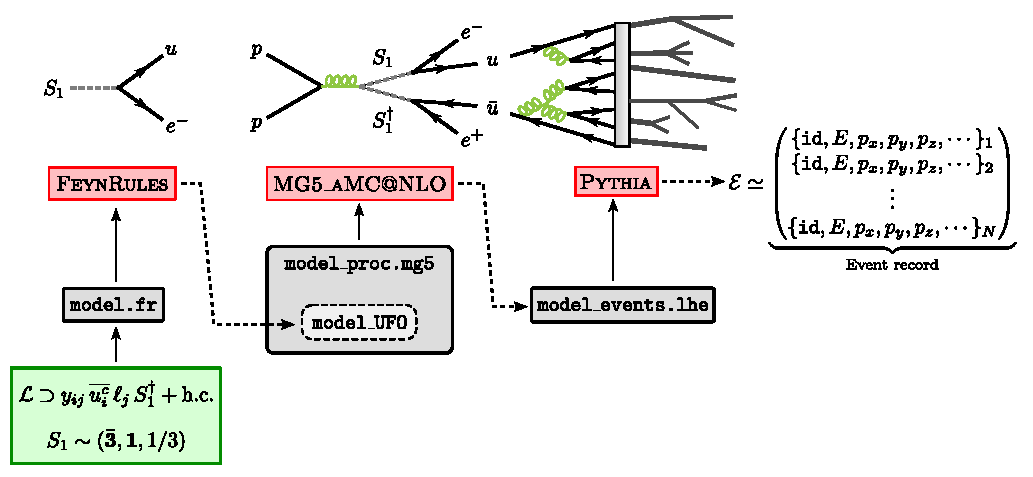
\includegraphics[width=0.97\textwidth]{figs/hep_workflow.pdf}
    \caption{
    One example of a multi-phase software workflow for a BSM leptoquark study. 
    A \texttt{model.fr} file is implemented in FeynRules and exported as a UFO directory (\texttt{model\_UFO/}). The UFO is consumed by \textsc{MG5\_aMC@NLO}, which loads the process card \texttt{model\_proc.mg5} and generates parton-level events written to \texttt{model\_events.lhe}. 
    These events are then passed to \textsc{Pythia} for showering and hadronization, producing an event record $\mathcal{E}$ containing particle identifiers and four-momenta $\{\,p_x, p_y, p_z, E, \texttt{id}, \ldots\}$. 
    }\label{fig:hep_workflow}
\end{figure}

For this example, a complete HEP workflow can be instantiated in several ways. One representative realization is considered here (see \cref{fig:hep_workflow}), though comparable pipelines using, for example, \textsc{Sherpa} \cite{Sherpa:2024mfk} follow the same basic structure:
\begin{enumerate}
    \item \textbf{Model generation:} convert the \textsc{FeynRules} \cite{Alloul:2013bka} model file into a Universal FeynRules Output (UFO) directory.
    \item \textbf{Parton-level event generation:} use \textsc{MadGraph5\_aMC@NLO} \cite{Alwall:2014hca} to generate events for each mass point specified in the run card via a user-defined parameter scan.
    \item \textbf{Showering and hadronization:} use \textsc{Pythia} 
    \cite{Bierlich:2022pfr} to process the LHE events into particle-level final states.
    \item \textbf{Jet reconstruction:} apply anti-\(k_T\) or Cambridge/Aachen clustering via \textsc{FastJet} \cite{Cacciari:2011ma}.
    \item \textbf{Resonance reconstruction:} pair leptons and jets, compute $m_{\text{LQ}}^{(1)}, m_{\text{LQ}}^{(2)}$, and derive $m^{\min}_{\text{LQ}}$.
\end{enumerate}

Careful management of run cards, file paths, tool configurations, and intermediate data formats is necessary to execute this sequence reliably. 
Manual pipelines are time-intensive and error-prone. 
In later sections we return to this example and show how \pkgname treats each phase as a schema-validated tool, propagates scan metadata through the workflow automatically, and uses run cards as explicit coordination boundaries. 
This allows an LLM to orchestrate the full analysis while preserving transparency, reproducibility, and human oversight.

\section{Orchestration architecture and philosophy}
\label{sec:architecture}

The central objective of \pkgname is to facilitate and enable large language models (LLMs) to reliably coordinate high-energy-physics (HEP) workflows while preserving transparency, reproducibility, and human oversight. 
The leptoquark workflow introduced in \cref{sec:example} highlights the central challenge in automating HEP analyses: while each individual phase of the pipeline is well supported by mature software packages, the coordination of these components remains largely manual. 
Researchers must construct run cards, manage intermediate files, ensure parameter consistency, and sequence tool execution correctly across multiple stages. 
These tasks are labor-intensive and error-prone, especially when extended across parameter scans or repeated for large model spaces.
The following subsections outline the architectural features of \pkgname that address these coordination challenges. 
A high-level view of the HEPTAPOD architecture and its interaction between agents, tools, and external HEP software is shown in \cref{fig:heptapod_workflow}.

\subsection{Schema-validated tools}
\label{subsec:schematools}

Each scientific capability in \pkgname is exposed to the agent as a \emph{tool}: a Python class with a structured JSON schema defining its inputs and outputs.
Tools serve as the fundamental interface between the agent and external HEP software. 
Within the orchestration framework, tools play three roles: 1.~to formalize how the agent invokes domain-specific capabilities, 2.~to return structured outputs that downstream steps can consume reliably, and 3.~to define clear execution boundaries that support reproducibility and human oversight. 

Tool schemas distinguish between \emph{runtime fields}, which the agent provides when invoking the tool, and \emph{state fields}, which are injected by the orchestration layer and not visible to the agent. 
Runtime fields correspond to the scientific and programmatic degrees of freedom, like relative paths, algorithmic configurations, and parameter choices. 
State fields supply environmental information such as workspace locations, internal defaults (\textit{e.g.}~dependency paths), or metadata from previous phases.
This separation keeps the agent's reasoning at the physics level while insulating it from unnecessary overhead from the details of the filesystem or workspace (\textit{a.k.a.}~sandbox).

A tool’s schema is defined directly by its class annotations, from which the orchestration layer derives validation rules that enforce argument conventions and ensure that all values exchanged between the agent and the execution environment are checked prior to tool execution. 
For example, a simplified \textsc{Pythia} interface might declare:
\begin{graybox}
    \begin{verbatim}
class PythiaFromRunCardTool(BaseTool):
    """
    Generate hadron-level events using Pythia8 from a .cmnd card.

    Inputs (runtime):
      - command_card: path to Pythia8 .cmnd configuration file
      - nevents: number of events to generate
      - seed: optional random seed
      ...

    Behavior:
      1. Initialize Pythia8 with the provided run card
      2. Generate nevents events with optional fixed seed
      3. Write structured event records to JSONL format
      ...

    Output (JSON):
      {"status": "ok", "events_jsonl": "<path>", ...}
    """
    # Runtime fields
    command_card: str = RuntimeField(
        description="Path to Pythia8 .cmnd configuration file")
    nevents: int = RuntimeField(
        description="Number of events to generate")
    seed: Optional[int] = RuntimeField(
        default=None, description="Random seed (optional)")
    \end{verbatim}
\end{graybox}

An agent invoking this tool submits a structured tool call, which is validated before execution. Schema validation prevents failures from those cases when runtime inputs do not satisfy the tool's declared interface. 
When failures do arise from external software (e.g. \textsc{FeynRules}, \textsc{MadGraph}, \textsc{Pythia}), tools return structured error objects that the agent can interpret and act upon. 
This provides predictable failure modes in place of unstructured logs.

As a design convention, tools also return structured JSON outputs. This ensures that each tool produces data in a form that downstream steps can consume without ad hoc parsing or heuristics. 
The output schema specifies the fields and their types, which guarantees that intermediate products such as UFO directories, LHE file paths, jet collections, or analysis summaries have a predictable structure. 
This removes ambiguity at tool boundaries and provides the agent with machine-checkable data structures rather than free-form text, which is essential for coordinating multi-step scientific workflows.
An example tool invocation and the associated JSON output for the \texttt{PythiaFromRunCardTool} is shown below:
\vspace{-0.2in}
\begin{minted}[escapeinside=||]{text}
PythiaFromRunCardTool(
    command_card="cards/run_ppbar.cmnd",
    nevents=5000,
    seed=12345
)
|$\to$| {"status": "ok", "events_jsonl": "data/run_01/events.jsonl", ...}
\end{minted}

Crucially, in addition to the schema itself, the \emph{tool docstring} (the Python docstring, a free-form text description attached to a function or class that explains what it does and how to use it) plays a critical role in guiding the agent's behavior. 
Each tool class carries a domain-specific docstring that describes its scientific purpose, the meaning of its runtime fields, expected behavior, and the semantics of its outputs.
This docstring functions as the tool's prompt: when the agent considers invoking the tool, the orchestration layer provides both the schema and the docstring, giving the agent a structured interface (the JSON schema) and a semantic interface (the natural-language description).
The tool docstring is extracted and included in the tool specification sent with every LLM API call, ensuring that the agent has immediate access to semantic context needed to understand what parameters to provide and how to interpret the returned fields without relying on conversational memory.
The combination is essential.
The schema tells the agent what inputs are allowed; the docstring tells the agent why and when the tool should be used.

Because outputs are returned as structured JSON, the tool docstring also defines the interpretation of those fields.
For example, the \textsc{MadGraph} tool docstring specifies that when a parameter scan is detected, the returned \texttt{runs} array contains objects with \texttt{run\_id}, \texttt{lhe\_file}, \texttt{scan\_params}, and \texttt{cross\_section} fields, where all file paths are relative to the sandbox.
This coupling between semantic guidance and machine-checkable structure enables the agent to reason about workflows without relying on free-form text generation or fragile pattern matching.
The agent uses the docstring to decide \emph{which} tool to invoke and the schema to decide \emph{how} to invoke it.

Together, the schema and the docstring act synergistically: the docstring communicates intent and scientific context; the schema enforces shape, type, and validity.
This is ultimately what allows tools to operate as reliable, composable units within multi-step workflows.

\subsection{LLM-compatible event data structures}
\label{subsec:evtjsonl}

Effective orchestration requires that intermediate physics data, particularly event-level outputs, be stored in a form that is both machine-actionable and directly interpretable by a language model, enabling the agent to participate meaningfully in validation, debugging, and exploratory analysis.
For this reason, \pkgname introduces a structured, text-based representation for intermediate event data, based on a line-delimited JSON (JSONL) format referred to throughout as the \texttt{evtjsonl} event format.

Traditional HEP event containers and event-record formats such as \textsc{Root} \cite{Antcheva:2009zz}, \textsc{HDF5}, \textsc{HepMC} \cite{Buckley:2019xhk} and \textsc{LHE} \cite{Alwall:2006yp} are optimized for storage density and I/O throughput in large scale simulation and analysis workflows.
While well suited to large-scale production and offline analysis, these formats are opaque to language models: they require specialized libraries for deserialization and expose internal structure only indirectly.
As a result, an LLM cannot inspect individual events, validate intermediate outputs, or reason about event content without invoking external tools.
In contrast, the JSONL representation encodes each event as a self-contained record that can be examined directly within the conversational context.
This allows the agent to inspect representative events, verify kinematic properties, and respond to qualitative queries about the data without leaving the orchestration layer.

The \texttt{evtjsonl} format standardizes this representation across all workflow stages while remaining intentionally extensible for future use cases (\textit{e.g.}~long-lived particle production, \textit{etc.}).
Each event record contains an \texttt{event\_id} field and a \texttt{data} object, which holds either a \texttt{particles} array for particle-level events or a \texttt{jets} array for reconstructed jet collections.
Particle objects include kinematic four-vectors $(p_x, p_y, p_z, E)$, mass $m$, PDG identifier \texttt{id}, and status codes; jet objects carry four-vectors and jet-specific metadata.
This uniform structure allows tools to consume event data predictably: all event generators, shower algorithms, jet clustering tools, and analysis selections produce and expect the same format, eliminating the need for ad hoc parsing or format conversions between workflow stages.

The line-delimited structure of JSONL also enables incremental processing.
Because each line is an independent record, tools can iterate through events sequentially, processing and writing results one event at a time without loading entire datasets into memory.
The format also simplifies parallelization and filtering: events can be distributed across workers or selected on-the-fly using standard command-line tools.
This design choice reflects a broader principle within \pkgname: intermediate data formats should be interpretable not only by the orchestration layer and downstream analysis tools, but also by the agent itself.

While JSONL sacrifices storage compactness relative to compressed formats, \pkgname mitigates this through interoperability tools.
\texttt{LHEToJSONLTool} imports Les Houches events from matrix-element generators; \texttt{EventJSONLToNumpyTool} and \texttt{JetsJSONLToNumpyTool} export to zero-padded NumPy arrays compatible with vectorized analysis libraries and machine-learning frameworks such as JAX, PyTorch, and TensorFlow.
This hybrid approach retains the agent-facing interpretability of JSONL during orchestration while enabling seamless integration with the broader HEP and ML ecosystems at analysis endpoints.

The uniform adoption of \texttt{evtjsonl} across the tool suite exemplifies a core design philosophy: data structures should be legible to both machines and agents, enabling the LLM to participate meaningfully in validation, debugging, and exploratory analysis.

\subsection{Run-card-driven orchestration}
\label{subsec:runcards}

Most major HEP collider simulation frameworks, including \textsc{FeynRules} \cite{Alloul:2013bka}, \textsc{MadGraph} \cite{Alwall:2011uj}, \textsc{Pythia} \cite{Bierlich:2022pfr}, \textsc{Sherpa} \cite{Sherpa:2024mfk}, \textsc{Herwig} \cite{Bewick:2023tfi}, \textsc{Delphes} \cite{deFavereau:2013fsa}, \textsc{Geant4} \cite{Allison:2016lfl}, and \textsc{Rivet} \cite{Bierlich:2019rhm}, are configured via human-readable run cards or model files. 
These declarative configuration files specify model parameters, beam conditions, detector settings, event-selection criteria, and analysis instructions. 
\pkgname adopts run cards as the canonical interface between the agent and external HEP codes because they provide a stable, interpretable, and versionable surface for steering scientific workflows.
Specifically, using run cards as the orchestration boundary provides three key advantages:
\paragraph{Reproducibility and transparency.}
Run cards define complete, standalone configurations that can be version-controlled, archived, and executed independently of the agent. Each decision made by the LLM is therefore captured in a persistent artifact, enabling fully auditable workflows.

\paragraph{Compatibility with RAG and structured prompting.}
Because run cards follow stable syntax conventions, they are highly amenable to retrieval-augmented generation (RAG). The agent can be contextualized with validated examples, available parameter dictionaries, and relevant excerpts from official manuals, allowing it to generate syntactically correct and meaningful configurations without memorizing the entire documentation. This reduces the likelihood of malformed configurations and improves the reliability of free-form prompting. 
We leave a full implementation of RAG-based run-card generation to future iterations of the framework.

\paragraph{Human-approval checkpoints.}
Each generated run card constitutes a natural boundary at which the researcher may inspect, modify, or approve the configuration before execution. This preserves scientific judgment while still benefiting from automated orchestration.

\subsection{Context propagation and stateful execution}
\label{subsec:context}

\pkgname maintains a structured conversation state or \emph{context} that records tool outputs and relevant metadata. Later steps can reference this state directly, rather than relying on the agent to recall filenames or parse textual logs. For example, when a run card includes a user-defined parameter scan (e.g., multiple values of a mass or coupling), the \textsc{MadGraph} tool automatically detects the scan structure by inspecting the resulting run directories for characteristic naming patterns (\textit{e.g.,}~\texttt{run\_01}, \texttt{run\_02}, \ldots) and parsing the scan summary files generated by \textsc{MadGraph}.
Instead of returning only LHE file paths, the tool produces structured metadata:
\medskip
\begin{graybox}
\begin{verbatim}
{ "scan_detected": true,
  "n_runs": 3,
  "runs": [
        {"run_id": "run_01", "lhe_file": "...", ...},
        {"run_id": "run_02", "lhe_file": "...", ...},
        {"run_id": "run_03", "lhe_file": "...", ...}
]}
\end{verbatim}
\end{graybox}
associating each scan point with its corresponding parameter values, file locations, and computed cross sections.
This metadata is written into the conversation state, allowing subsequent steps, such as \textsc{Pythia}, to access the scan information directly without requiring the agent to interpret directory names or rely on textual recall.

Additionally, tools automatically detect and substitute placeholder values in run cards at execution time.
For instance, a \textsc{MadGraph} command card may contain \texttt{import model [[UFO\_PATH]]}, or a \textsc{Pythia} configuration may specify \texttt{Beams:LHEF = [[LHEF\_PATH]]}.
When invoked, the corresponding tool identifies these bracketed placeholders and replaces them with the actual file paths supplied as arguments (\textit{e.g.,}~the UFO directory from \textsc{FeynRules} output or the LHE file from a specific scan point):
\medskip
\begin{graybox}
\begin{verbatim}
# Template run card
Beams:LHEF = [[LHEF_PATH]]

# Automatically becomes
Beams:LHEF = data/mg_run001/.../run_01/events.lhe.gz
\end{verbatim}
\end{graybox}
This eliminates the need for agents to manually edit configuration files or construct fragile string-replacement logic, enabling run cards to serve as reusable templates across different workflow invocations while maintaining full traceability of substituted values in the execution log. 

Together, schema-validated tools, stateful context propagation, and run-card-driven orchestration provide a robust foundation for LLM-assisted workflows. 
These mechanisms ensure that multi-stage HEP analyses remain interpretable, reproducible, and aligned with established scientific practice.

\begin{figure}[t!]
    \centering
    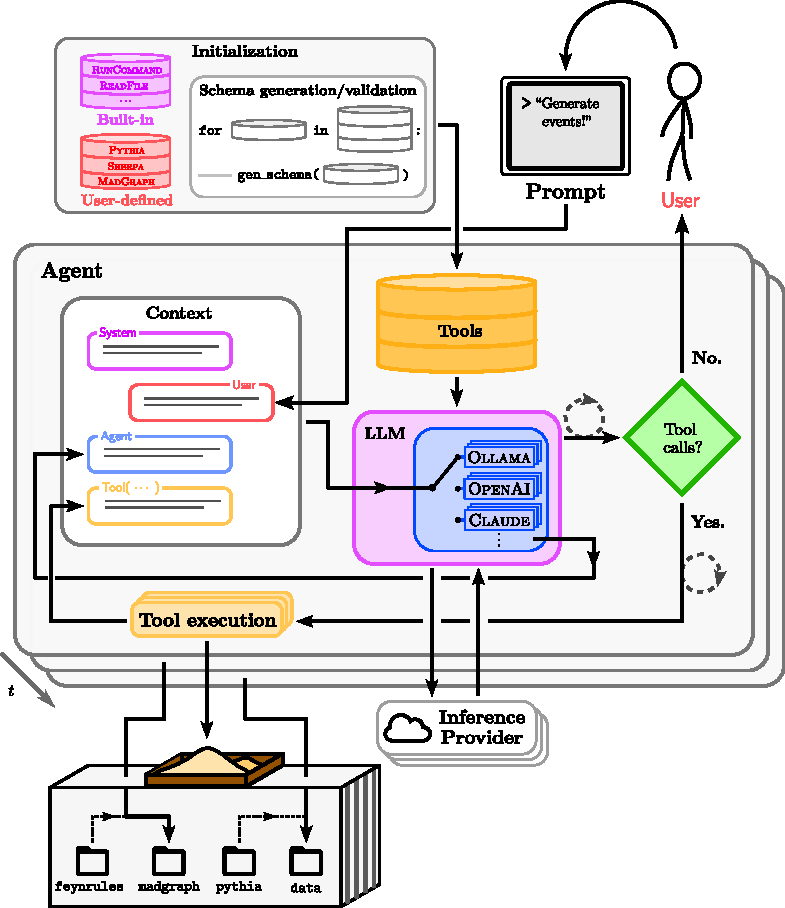
\includegraphics[width=0.81\textwidth]{figs/heptapod_diagram.pdf}
    \caption{
    High-level architecture of \pkgname, a HEP-focused agent-orchestration framework built using the \textsc{Orchestral AI} orchestration engine \cite{orchestral-ai}. The system consists of three interacting components: \textbf{(i)} a database of schema-validated tools that expose domain-specific HEP capabilities via structured inputs and outputs; \textbf{(ii)} an agent-orchestration layer that maintains the evolving context and performs LLM-based reasoning, optionally routing inference across multiple providers; and \textbf{(iii)} a sandboxed tool-execution engine that interfaces with external HEP software and data utilities. 
    Each agent interaction proceeds within an initialized sandboxed workspace, with the agent iteratively reasoning over the evolving context.
    At each step, the agent determines whether a tool invocation is required; when invoked, tools are executed outside the LLM within the sandbox, and their structured outputs (e.g.\ JSON artifacts) are injected back into the context before the next reasoning step. This closed-loop reasoning–execution process enables reliable, multi-step HEP workflows while enforcing a strict separation between language-model reasoning and external software execution.
    }\label{fig:heptapod_workflow}
\end{figure}

\subsection{Orchestration versus scripting}

Before turning to a full workflow demonstration, it is useful to contrast the orchestration model with traditional scripting approaches commonly used to automate HEP simulations.

While scripting remains the standard approach for automating HEP workflows, it imposes important structural constraints. 
A bash script or Python pipeline can sequentially invoke \textsc{FeynRules}, \textsc{MadGraph}, \textsc{Pythia}, and downstream analysis tools. 
However, scripting enforces static control flow: parameters, file paths, and branching logic are embedded directly in code. 
As a result, adapting a workflow such as changing scan configurations, modifying analysis logic, or responding to tool failures requires manual intervention and re-editing of implementation details. 
Moreover, scripts provide no formal mechanism for representing workflow intent or ensuring consistency of metadata across heterogeneous tools.
These structural limitations can be alleviated through the introduction of an explicit orchestration layer with the following properties:

\paragraph{Adaptive workflow construction.}
Workflows are specified at the level of physics intent rather than program control flow. 
The LLM constructs executable plans by selecting appropriate tool invocations, propagating run-card metadata, and managing multi-stage execution. 
This approach decouples workflow specification from its implementation, enabling dynamic reconfiguration without modifying underlying code.

\paragraph{Structured error interpretation and recovery.}
Each tool exposes a schema-defined interface that includes structured failure modes. 
Instead of unstructured log output, tools return machine-interpretable error objects that the LLM can analyze to propose corrective actions or request clarification. This yields more resilient execution patterns and facilitates automated recovery strategies under human supervision.

\paragraph{Workflow transparency and provenance.}
Tool invocations and their outputs form an explicit execution trace, providing a machine-readable record of workflow decisions and intermediate artifacts. This provenance layer supports reproducibility, auditability, and collaboration, and is difficult to achieve in traditional scripts without significant custom infrastructure.

These capabilities introduce additional abstraction layers and rely on LLM reasoning quality, so for fixed or static pipelines, scripting may remain adequate. For exploratory analyses, parameter-dependent workflows, and multi-stage simulation studies, the orchestration layer provides stronger guarantees of adaptability, consistency, and traceability.

The following section returns to the leptoquark analysis introduced in \cref{sec:example} and illustrates these mechanisms in practice via a complete, multi-stage workflow orchestrated with \pkgname, showing how an agent constructs, executes, and analyzes a realistic HEP pipeline.

\section{Agent-orchestrated workflow}
\label{sec:example_full}

We now demonstrate how the \pkgname tool suite operates in practice by presenting an end-to-end execution of the leptoquark mass-scan workflow introduced in \cref{sec:example}. 
The goal is to illustrate how an agent, equipped with the orchestration mechanisms of \cref{sec:architecture}, constructs and executes a multi-stage HEP pipeline inside a pre-initialized sandbox while maintaining transparency, reproducibility, and human oversight. 

For concreteness, we retain the simplifying assumptions of the running example and consider a first-generation-philic scalar leptoquark with diagonal couplings to $(u,e)$, scanning over three benchmark mass points. 
The physics content of the example is unchanged; the focus here is the interaction between the agent and the orchestration layer.

\vspace{0.5em}
\noindent\textbf{Interaction modes}
Within the orchestration framework, there are several patterns of possible interaction between the user and the agent, each corresponding to a different level of planning autonomy. These modes share the same tool suite and execution environment but differ in how workflow intent is specified:

\begin{itemize}
  \item \textbf{To-do mode.}
  The user supplies a predefined, phase-structured to-do list (\texttt{todos.md}) describing the full workflow. 
  The agent executes tasks sequentially, updating task status and advancing through the prescribed stages with minimal additional input. This is closest to “programming” the workflow directly.

  \item \textbf{Planner mode.}
  The user provides a high-level objective. The agent autonomously constructs an explicit, step-by-step plan after inspecting the sandbox (model files, run cards, directory structure).
  The agent then executes this plan, invoking tools and verifying outputs at each stage. 
  This mode highlights the planning and coordination capabilities enabled by schema-validated tools and run-card-driven configuration.

  \item \textbf{Explorer mode.}
  A general interactive mode in which the agent responds to user queries or instructions without producing a global plan. 
  This mode is useful for exploratory tasks, debugging, or incremental development of workflows.
\end{itemize}


Each conversation begins in a containerized sandbox, initialized with the relevant model files and run cards provided by the user. 
As the workflow proceeds, tools populate this workspace with intermediate and final output (UFO directories, LHE files, JSONL event streams, jets, reconstructed observables).
In \cref{subsec:example_convo}, the sandbox is initialized with the following directory structure:
\begin{orchestralsystemmessage}

\begin{minted}{text}
.
├── feynrules
│   └── models
│       └── S1_LQ_RR.fr
├── madgraph
│   └── cards
│       └── S1_LQ_RR_pp_lqlq_scan.mg5
└── pythia
    └── cards
        └── S1_LQ_RR_pp_ljlj.cmnd

7 directories, 3 files
\end{minted}
    \end{orchestralsystemmessage}
where \texttt{S1\_LQ\_RR.fr}, \texttt{S1\_LQ\_RR\_pp\_lqlq\_scan.mg5}, and \texttt{S1\_LQ\_RR\_pp\_ljlj.cmnd} are assumed to be syntactically valid model files/run cards for \textsc{FeynRules}, \textsc{MadGraph}, and \textsc{Pythia}, respectively.
In to-do mode conversations, a user-defined todo-list is also copied into the sandbox.

\subsection{Example conversation}
\label{subsec:example_convo}


Below we provide an annotated transcript of a ``planning'' conversation with a GPT-OSS-120B \cite{openai2025gptoss120bgptoss20bmodel} agent. 
Throughout this example, the agent operates over pre-existing, syntactically valid \textsc{FeynRules}, \textsc{MadGraph}, and \textsc{Pythia} model files and run cards, managing their invocation, parameterization, and file-level dependencies rather than constructing the run cards themselves.
Note that some tool invocations and outputs are simplified for pedagogical clarity and brevity. 
Importantly, while this transcript shows only the JSON outputs returned by tools, the agent receives the full tool docstring (describing inputs, outputs, and scientific semantics) with each API call as described in \cref{sec:architecture}. 
For completeness, \cref{app:tools} provides a brief summary of each tool and its primary use case, while the full tool docstrings are available in the public code repository.

\textbf{The system prompt.}
Conversational language models take as input a \emph{context} consisting of a structured list of messages with various roles such as \emph{user} or \emph{assistant}. 
Many frameworks also support specialized roles for \emph{tool} responses, and for \emph{system} messages. 
LLMs are generally fine tuned to strictly follow instructions given to them in these system messages. 
Most conversations begin with a ``system prompt'': a system message which shapes the LLM's behavior and can be used to define specialized context, goals, guidelines, formatting requirements, and operational constraints.
When using LLMs, one typically either needs to explicitly manage the context and append new messages, or use a framework which handles this. 
We implement our agents with \orchestralai, which automatically manages the context while allowing us to define our own custom system prompt.
The example below uses the following system prompt:

\begin{orchestralsystemmessage}
    You are a helpful assistant, expert high-energy-physicist, and professional computational scientist running on the Orchestral AI platform.
    Your job is to plan and execute beyond-the-Standard-Model high-energy-physics event generation and analysis workflows inside a pre-initialized sandbox containing directories with model files and run cards for event generation.
    Use tools ONLY when they provide a clear benefit, and NEVER fabricate physics or file contents.
    Markdown and LaTeX are allowed. Escape dollar signs except in math. No emojis.
    \vspace{0.05in}
    \begin{enumerate}
    \item \textbf{Workspace model}\\
    At the start of a session:
    \begin{enumerate}
        \item List the top-level directories and files.
        \item Inspect representative files with \texttt{readfile} to identify:\\
            -- which are model directories,\\
            -- which contain model files (\texttt{.fr}) or run cards (\texttt{.mg5}, \texttt{.cmnd}),\\
            -- collider configuration (beam type, energy),\\
            -- mass and coupling definitions.
    \end{enumerate}
    Treat these files as authoritative. Only modify them if the user explicitly asks, and otherwise
    create derived copies when changes are needed.
    \vspace{0.05in}
    \item \textbf{Workflow planning protocol}\\
    Your primary responsibility is structured planning followed by execution.\\
    \textit{Step 1: Clarify the goal}\\
    Summarize the user's objective in 1-3 sentences (e.g., event generation, validation, plotting).
    If already clear from context, restate without asking.

    \textit{Step 2: Write an explicit todo list}\\
    Create a to do list with concise steps that typically include:
    \begin{enumerate}
        \item Parameter selection and BSM model file generation.
        \item Event generation using the appropriate run card.
        \item Showering/hadronization.
        \item Analysis tasks (clustering, invariant masses, histograms).
        \item Plotting and summary outputs.
    \end{enumerate}

    \textit{Step 3: Execute step-by-step}\\
    For each planned step:
    \begin{enumerate}
        \item Invoke the correct tool with explicit arguments.
        \item Verify outputs (existence or small summary inspection).
        \item Provide a short progress message and proceed to the next step.
    \end{enumerate}
    \textit{\textbf{Work autonomously}} -- proceed through phases without waiting for the user.
    \vspace{0.05in}
    \item \textbf{Physics and workflow constraints}\\
    -- Do not alter collider settings unless instructed.\\
    -- Provide minimal run metadata after major tasks (inputs, seeds, versions).\\
    -- Give qualitative physics interpretations only; avoid strong claims without explicit
    statistical instruction.
\end{enumerate}

    % \vspace{0.5em}
    \centerline{\vdots}
    \vspace{0.5em}

\end{orchestralsystemmessage}

\noindent
\textbf{The user prompt.}
Since LLM APIs operate as user-facing oracles, they require an explicit user prompt to generate a streamed response; the system prompt is transmitted implicitly and is not exposed to the API until the user submits the first prompt.

\begin{orchestralusermessage}
    Plan a Monte Carlo signal-validation analysis of the BSM scalar leptoquark defined by the supplied run cards. 
    Generate 10,000 events, select objects, and create lepton-jet invariant-mass distributions for each parameter point.
    Attempt to isolate and reconstruct the leptoquark resonance by applying reasonable lepton-jet separation and experimental cuts. 
    Compute and plot the resulting $m^{\text{min}}_{\text{LQ}}$ distribution. 
    Write a todo list first and then execute the todo list until completed.
\end{orchestralusermessage}

The agent responds by first recursively listing its current workspace:

\begin{orchestralagentmessage}


    \begin{orchestraltoolmessage}{RunCommand( \texttt{command=ls -R ., timeout=120000} )}
\begin{minted}{text}
Command: ls -R .
Return Code: 0
Output:
feynrules    madgraph    pythia

./feynrules:
models
./feynrules/models:
S1_LQ_RR.fr
./madgraph:
cards
./madgraph/cards:
S1_LQ_RR_pp_lqlq_scan.mg5
./pythia:
cards
./pythia/cards:
S1_LQ_RR_pp_ljlj.cmnd
\end{minted}
    \end{orchestraltoolmessage}

\end{orchestralagentmessage}
followed by the generation of a markdown todo list using the \texttt{TodoWriteTool}. The first item, marked with \texttt{[*]}, denotes that the task is in-progress.
\begin{orchestralagentmessage}

    \begin{orchestraltoolmessage}{ToDoWrite}
        \textbf{Todos:}\vspace{-0.2in}
\begin{minted}{text}
## Monte Carlo Signal-Validation Analysis for S1 Leptoquark

- [*] Generate UFO model from FeynRules file 
      `feynrules/models/S1_LQ_RR.fr`
- [ ] Generate parton-level events with MadGraph using card 
      `madgraph/cards/S1_LQ_RR_pp_lqlq_scan.mg5`
    - set `nevents = 10000`
    - keep all parameter points
- [ ] Shower and hadronize events with Pythia using card 
      `pythia/cards/S1_LQ_RR_pp_ljlj.cmnd`
    - `shower_lhe = True`
- [ ] Convert Pythia JSONL events to NumPy array
- [ ] Apply kinematic cuts to leptons and jets
    - leptons: pt>20 GeV, |eta|<2.5, PDG IDs 11,13 (and charge 
      conjugates)
    - jets: pt>30 GeV, |eta|<2.5
- [ ] Select hardest 2 leptons and hardest 2 jets per event
- [ ] Compute lepton-jet invariant masses for all pairings and retain
      the minimum per event (`m^min_{LQ}`)
- [ ] Plot the `m^min_{LQ}` distribution (histogram, 50 bins, 
      appropriate range) and save as `mmin_LQ.png`
- [ ] Summarize results (number of events, cross-section, plot 
      location)
\end{minted}
    \end{orchestraltoolmessage}
\end{orchestralagentmessage}
The todo list then proceeds through the event-generation tool chain, beginning with UFO model generation in \textsc{FeynRules}, followed sequentially by parton-level event generation with \textsc{MadGraph} and showering and hadronization with \textsc{Pythia}:
\begin{orchestralagentmessage}
    \begin{orchestraltoolmessageml}{FeynRulesToUFO( \texttt{model\_path=feynrules/models/S1\_LQ\_RR.fr,} \\\hphantom{FeynRulesToUFO(}
        \texttt{output\_dir=feynrules/models/S1\_LQ\_RR\_UFO,}\\\hphantom{FeynRulesToUFO(}
        \texttt{timeout\_sec=1800} )
    }

    \textbf{Output logs:} \vspace{-0.2in}
        \begin{minted}[escapeinside=||]{text}
{
    "schema_version": "tool-1.0",
    "ok": true,
    "model_path": "feynrules/models/S1_LQ_RR.fr",
    "output_dir": "feynrules/models/S1_LQ_RR_UFO",
    "wolframscript_path": "<path/to/wolframscript>",
    "feynrules_path": "<path/to/feynrules>",
    "logs": {
    "stdout": "feynrules/models/S1_LQ_RR_UFO/_logs/wolframscript_stdout.log",
    "stderr": "feynrules/models/S1_LQ_RR_UFO/_logs/wolframscript_stderr.log"
    },
    "files_created": [
    "couplings.py",
    "decays.py",
    "lorentz.py",
    "parameters.py",
    "particles.py",
    "propagators.py",
    "vertices.py",
         |$\vdots$|
    ]
}
        \end{minted}
    \end{orchestraltoolmessageml}


    \begin{orchestraltoolmessage}{ReadFile( \texttt{limit=200, path=madgraph/cards/S1\_LQ\_RR\_pp\_lqlq.mg5} )}
    \begin{minted}[escapeinside=||]{text}
File: madgraph/cards/S1_LQ_RR_pp_lqlq_scan.mg5 (35 lines)
 1→ set automatic_html_opening False
 2→ 
 3→ # Load the Standard Model UFO (built in)
 4→ import model [[UFO_PATH]]
 5→ 
 6→ # Define beam contents (proton = quarks + gluon)
 7→ define p = g u c d s b u~ c~ d~ s~ b~
 8→ 
10→ # Define a simple process:
11→ generate p p > S1 S1~, (S1 > e- u), (S1~ > e+  u~)
12→                     |$\vdots$|
    \end{minted}
    \end{orchestraltoolmessage}


    \begin{orchestraltoolmessageml}{MadgraphFromRunCard(\texttt{run\_card=<path/to>/S1\_LQ\_RR\_pp\_lqlq.mg5, nevents=10000} \\\hphantom{MadgraphFromRunCard(}\texttt{data\_dir=data/mg\_run001, output=S1\_LQ\_scan,}\\\hphantom{MadgraphFromRunCard(}\texttt{ufo\_path=feynrules/models/S1\_LQ\_RR\_UFO} )}
        \textbf{Output logs:} \vspace{-0.2in}
\begin{minted}[escapeinside=||]{text}
{"status":"ok",
"scan_detected":true,"data_dir":"data/mg_run001",
"lhe_file":"data/mg_run001/S1_LQ_scan/Events
            /run_01/unweighted_events.lhe.gz",
"manifest_json":"data/mg_run001/manifest.json",
"log_file":"data/mg_run001/mg5_run.log",
"scan_summary_file":"data/mg_run001/S1_LQ_scan/Events
                     /scan_run_0[1-3].txt",
"n_runs":3,
"runs":[
        {"run_id":"run_01",
         "lhe_file":"data/mg_run001/S1_LQ_scan/Events/
                     run_01/unweighted_events.lhe.gz",
         "scan_params":{"mass#9000005":1000.0},
         "cross_section":0.1016761,
         "cross_section_error":0.0001923201},
        {"run_id":"run_02",
         "lhe_file":"data/mg_run001/S1_LQ_scan/Events/
                     run_02/unweighted_events.lhe.gz",
         "scan_params":{"mass#9000005":1500.0},
         "cross_section":0.008729035,
         "cross_section_error":1.541146e-05},
                          |$\vdots$|
        ]
    }
\end{minted}
    \end{orchestraltoolmessageml}


    \begin{orchestraltoolmessage}{ReadFile( \texttt{limit=200, path=pythia/cards/S1\_LQ\_RR\_pp\_ljlj.cmnd} )}
\begin{minted}{text}
File: pythia/cards/S1_LQ_RR_pp_ljlj.cmnd (11 lines)
 1→ #------------------------------------------------------------
 2→ # Example: pp_S1S1d_ljlj.cmnd
 3→ # Minimal Pythia8 run card to shower LHE events from MadGraph
 4→ #------------------------------------------------------------
 5→ 
 6→ # Beam and input setup
 7→ Beams:frameType = 4
 8→ Beams:LHEF      = [[LHEF_PATH]]
 9→ 
10→ # Quiet output
11→ Print:quiet = on
\end{minted}
    \end{orchestraltoolmessage}


    \begin{orchestraltoolmessageml}{PythiaFromRunCard(\texttt{ cmnd\_path="pythia/cards/S1\_LQ\_RR\_pp\_ljlj.cmnd",}\\\hphantom{PythiaFromRunCard(} 
    \texttt{data\_dir="data/pythia\_run01", finals\_only="True",}\\\hphantom{PythiaFromRunCard(} \texttt{lhe\_path="<path/to>/run\_01/unweighted\_events.lhe.gz", ... )}}
        \textbf{Output logs:}\vspace{-0.2in}

\begin{minted}{text}
{"status":"ok",
"data_dir":"data/pythia_run01",
"events_jsonl":"data/pythia_run01/events.jsonl",
"manifest_json":"data/pythia_run01/manifest.json",
"accepted":10000,
"failed":0}
\end{minted}
    \end{orchestraltoolmessageml}


    \begin{orchestraltoolmessage}{PythiaFromRunCard( $\cdots$ )}
        Same as above with \texttt{run\_01} $\to$ \texttt{run\_02}
    \end{orchestraltoolmessage}

    \begin{orchestraltoolmessage}{PythiaFromRunCard( $\cdots$ )}
        Same as above with \texttt{run\_02} $\to$ \texttt{run\_03}
    \end{orchestraltoolmessage}


    \begin{orchestraltoolmessageml}{JetClusterSlowJet( \texttt{R=0.4, algorithm=antikt, cluster\_all=True, etamax=5,}\\\hphantom{JetClusterSlowJet(}
         \texttt{jsonl\_path=data/pythia\_run01/events.jsonl, mass\_option=1,}\\\hphantom{JetClusterSlowJet(} \texttt{output\_path=data/pythia\_run01/jets.jsonl, ptmin=0} )}
\begin{minted}{text}
{"status":"ok",
"n_events":10000,
"output_file":"data/pythia_run01/jets.jsonl"}
\end{minted}
    \end{orchestraltoolmessageml}

    \begin{orchestraltoolmessage}{JetClusterSlowJet( $\cdots$ )}
        Same as above with \texttt{run\_01} $\to$ \texttt{run\_02}
    \end{orchestraltoolmessage}

    \begin{orchestraltoolmessage}{ToDoWrite}
        \textbf{Todos:}\vspace{-0.2in}

\begin{minted}{text}
## Monte Carlo Signal‑Validation Analysis for S1 Leptoquark

- [x] Generate UFO model from FeynRules file 
      `feynrules/models/S1_LQ_RR.fr`
- [x] Generate parton‑level events with MadGraph using card 
      `madgraph/cards/S1_LQ_RR_pp_lqlq_scan.mg5`
    - set `nevents = 10000`
    - keep all parameter points
- [x] Shower and hadronize events with Pythia using card 
      `pythia/cards/S1_LQ_RR_pp_ljlj.cmnd`
    - `shower_lhe = True`
- [x] Cluster jets for each run
    - run01 jets `data/pythia_run01/jets.jsonl`
    - run02 jets `data/pythia_run02/jets.jsonl`
    - run03 jets `data/pythia_run03/jets.jsonl`
- [*] Select hardest objects and compute m^min_{LQ}
    - select hardest 2 leptons (pdg 11, -11, 13, -13) per event
    - select hardest 2 jets per event
    - compute invariant masses for all lepton-jet pairings, 
      keep minimum per event
    - plot histogram of m^min_{LQ} (50 bins) and save as 
      `mmin_LQ.png`
- [ ] Summarize results (event counts, cross-sections, 
      plot location)
\end{minted}
    \end{orchestraltoolmessage}


    \begin{orchestraltoolmessageml}{FilterByPDGID(  \texttt{input\_path=data/pythia\_run01/events.jsonl,}\\
        \hphantom{FilterByPDGID(} \texttt{output\_path=data/pythia\_run01/leptons\_all.jsonl,}\\\hphantom{FilterByPDGID(}
        \texttt{pdgids=[11, -11, 13, -13]} )}
\begin{minted}{text}
{"status":"ok",
"input_events":10000,
"particles_before":5241292,
"particles_after":54846,
"kept_pdgids":[11,-11,13,-13],
"output_path":"data/pythia_run01/leptons_all.jsonl"}
\end{minted}
    \end{orchestraltoolmessageml}


    \begin{orchestraltoolmessageml}{GetHardestN( \texttt{input\_path=data/pythia\_run01/leptons\_a.ll.jsonl,}\\
        \hphantom{GetHardestN(}
         \texttt{n\_hardest=2,}\\
        \hphantom{GetHardestN(} \texttt{output\_path=data/pythia\_run01/hardest2\_leptons.jsonl} )}
\begin{minted}{text}
{"status":"ok",
"input_events":10000,
"n_hardest":2,
"output_path":"data/pythia_run01/hardest2_leptons.jsonl"}
\end{minted}
    \end{orchestraltoolmessageml}


    \begin{orchestraltoolmessageml}{GetHardestNJets(  \texttt{input\_path=data/pythia\_run01/jets.jsonl,}\\\hphantom{GetHardestNJets(} 
        \texttt{n\_hardest=2,}\\\hphantom{GetHardestNJets(}
        \texttt{output\_path=data/pythia\_run01/hardest2\_jets.jsonl} )}
\begin{minted}{text}
{"status":"ok",
"input_events":10000,
"n_hardest":2,
"output_path":"data/pythia_run01/hardest2_jets.jsonl"}
\end{minted}
    \end{orchestraltoolmessageml}


    \begin{orchestraltoolmessageml}{ResonanceReconstruction( \texttt{min\_delta\_r=0.4, output\_prefix=outputs/run01\_LQ,}\\\hphantom{ResonanceReconstruction(} \texttt{particle\_arrays=[<path/to>/hardest2\_leptons.jsonl, ...]}\\\hphantom{ResonanceReconstruction(}
    \texttt{template=two\_body\_symmetric} )}
\begin{minted}{text}
{"status":"ok",
"template":"two_body_symmetric",
"n_arrays":2, ...
"n_events_analyzed":10000,
"n_events_successful":9830, ...,
"observables":[...],
"histograms":[{"observable":"m1",
"bins":[...], "counts":[...]},
{"observable":"m2",
"bins":[...], "counts":[...]},
{"observable":"m_min",
"bins":[...], "counts":[...]},
{"observable":"m_max",
"bins":[...],
"counts":[...]}],
"data_paths":{...,
"m_min":"outputs/run01_LQ_m_min.npy",
"m_max":"outputs/run01_LQ_m_max.npy"}}
\end{minted}
    \end{orchestraltoolmessageml}


    \begin{orchestraltoolmessage}{ReadFile( \texttt{limit=200, path=data/mg\_run001/manifest.json} )}
\begin{minted}[escapeinside=||]{text}
File: data/mg_run001/manifest.json (20 lines)
                                    |$\vdots$|
\end{minted}
    \end{orchestraltoolmessage}


    \begin{orchestraltoolmessage}{FilterByPDGID( $\cdots$ )
        }
    Same as \textsf{FilterByPDGID} above with \texttt{run\_01} $\to$ \texttt{run\_02}
    \end{orchestraltoolmessage}


    \begin{orchestraltoolmessage}{FilterByPDGID( $\cdots$ )
        }
    Same as \textsf{FilterByPDGID} above with \texttt{run\_02} $\to$ \texttt{run\_03}
    \end{orchestraltoolmessage}


    \begin{orchestraltoolmessage}{GetHardestN( $\cdots$ )}
    Same as \textsf{GetHardestN} above with \texttt{run\_01} $\to$ \texttt{run\_02}
    \end{orchestraltoolmessage}

    \begin{orchestraltoolmessage}{GetHardestNJets( $\cdots$ )}
    Same as \textsf{GetHardestNJets} above with \texttt{run\_01} $\to$ \texttt{run\_02}
    \end{orchestraltoolmessage}

    \begin{orchestraltoolmessageml}{ResonanceReconstruction( \texttt{min\_delta\_r=0.4, output\_prefix=outputs/run02\_LQ,}\\\hphantom{ResonanceReconstruction(} \texttt{particle\_arrays=['data/pythia\_run02/hardest...,}\\\hphantom{ResonanceReconstruction(}
    \texttt{template=two\_body\_symmetric}}
\begin{minted}[escapeinside=||]{text}
|\textcolor{red}{Error: Processing Error}|
- Reason: Array 1 not found: data/pythia_run02/hardest2_jets.jsonl
\end{minted}
    \end{orchestraltoolmessageml}

    \begin{orchestraltoolmessageml}{GetHardestNJets(  \texttt{input\_path=data/pythia\_run03/jets.jsonl,}\\\hphantom{GetHardestNJets(} 
            \texttt{n\_hardest=2,}\\\hphantom{GetHardestNJets(}
            \texttt{output\_path=data/pythia\_run03/hardest2\_...}}
\begin{minted}[escapeinside=||]{text}
|\textcolor{red}{Error: File Not Found}|
- Reason: Input file not found: data/pythia_run03/jets.jsonl
\end{minted}
    \end{orchestraltoolmessageml}

    \begin{orchestraltoolmessage}{JetClusterSlowJet( $\cdots$ )}
        Same as above with \texttt{run\_02} $\to$ \texttt{run\_03}
    \end{orchestraltoolmessage}

    \begin{orchestraltoolmessage}{GetHardestN( $\cdots$ )}
    Same as \textsf{GetHardestN} above with \texttt{run\_02} $\to$ \texttt{run\_03}
    \end{orchestraltoolmessage}


    \begin{orchestraltoolmessage}{GetHardestNJets( $\cdots$ )}
    Same as \textsf{GetHardestNJets} above with \texttt{run\_02} $\to$ \texttt{run\_03}
    \end{orchestraltoolmessage}


    \begin{orchestraltoolmessage}{ResonanceReconstruction( $\cdots$ )}
    Retry of \texttt{run\_02}
    \end{orchestraltoolmessage}

\begin{orchestraltoolmessage}{ResonanceReconstruction( $\cdots$ )}
    Same as \textsf{ResonanceReconstruction} above with \texttt{run\_02} $\to$ \texttt{run\_03}
    \end{orchestraltoolmessage}

\end{orchestralagentmessage}

In the above tool chain, note the automated error-handling behavior that occurs when the agent incorrectly assumes that jet clustering had already been completed for all scan points. 
The tool execution layer returns a structured error, enabling the agent to identify and correct the missing step rather than encountering an opaque runtime failure that would typically terminate a conventionally scripted workflow. 
The agent responds by re-invoking the appropriate jet-clustering step for the affected run before successfully resuming resonance reconstruction. 
Finally, the agent finishes execution by generating the requested plot and summarizing the results.

\begin{orchestralagentmessage}

    \begin{orchestraltoolmessage}{RunPython}
        \textbf{Code:}\vspace{-0.2in}

        \begin{minted}{python}
    import subprocess, os, sys, json, numpy as np, matplotlib.pyplot as plt

    # Ensure matplotlib backend for headless
    import matplotlib
    matplotlib.use('Agg')

    paths = {
        '1000 GeV': 'outputs/run01_LQ_m_min.npy',
        '1500 GeV': 'outputs/run02_LQ_m_min.npy',
        '2000 GeV': 'outputs/run03_LQ_m_min.npy'
    }

    data = {label: np.load(p) for label,p in paths.items()}

    plt.figure(figsize=(8,6))
    for label, arr in data.items():
        plt.hist(arr, bins=50, histtype='step', label=label)
    plt.xlabel('m_{min}^{LQ} [GeV]')
    plt.ylabel('Events')
    plt.title('Minimum lepton‑jet invariant mass per event')
    plt.legend()
    plt.grid(True)
    plt.tight_layout()
    plt.savefig('mmin_LQ.png')
    print('Plot saved to mmin_LQ.png')

        \end{minted}

        \textbf{Output:}\vspace{-0.2in}

        \begin{minted}{text}
    {"stdout": "Plot saved to mmin_LQ.png", "stderr": "", "return_code": 0}
        \end{minted}
    \end{orchestraltoolmessage}

    \vspace{0.1in}

    \textbf{Completed workflow:}

    \begin{center}
    \begin{tabularx}{\textwidth}{p{1cm} X X}
    \hline
    \textbf{Step} & \textbf{Description} & \textbf{Outcome} \\
    \hline
    1 & Generate UFO model from \texttt{feynrules/models/S1\_LQ\_RR.fr} & UFO created in \texttt{feynrules/models/S1\_LQ\_RR\_UFO} \\
    2 & Generate parton-level events with MadGraph (3 scan points: 1000 GeV, 1500 GeV, 2000 GeV) & 10,000 LHE events per point (\texttt{data/mg\_run001/...}) \\
    3 & Shower \& hadronize with Pythia8 (\texttt{pythia/cards/S1\_LQ\_RR\_pp\_ljlj.cmnd}) & 10,000 final-state events per point (\texttt{data/pythia\_run0X/events.jsonl}) \\
    4 & Jet clustering (anti-$k_t$ $R=0.4$) & Jets stored in \texttt{data/pythia\_run0X/jets.jsonl} \\
    5 & Lepton selection (electrons $\pm 11$, muons $\pm 13$) & \texttt{leptons\_all.jsonl} for each run \\
    6 & Keep hardest 2 leptons \& hardest 2 jets per event & \texttt{hardest2\_leptons.jsonl}, \texttt{hardest2\_jets.jsonl} \\
    7 & Reconstruct leptoquark candidates (two-body symmetric template, $\Delta R > 0.4$) & Minimum lepton-jet invariant mass $m_{\text{min}}$ saved as NumPy arrays \texttt{outputs/run0X\_LQ\_m\_min.npy} \\
    8 & Plot the distribution of $m^{\text{min}}_{\text{LQ}}$ for the three mass points & Histogram saved as \texttt{mmin\_LQ.png} \\
    9 & Summarize results & See below \\
    \hline
    \end{tabularx}
    \end{center}
    \vspace{0.1in}
    
    \textbf{Plot}

    \vspace{0.1in}
    The file \texttt{mmin\_LQ.png} contains over-laid histograms (50 bins) of the minimum lepton-jet invariant mass per event for the three leptoquark mass hypotheses (1000 GeV, 1500 GeV, 2000 GeV). The peaks shift upward with the leptoquark mass, demonstrating successful reconstruction.

    \vspace{0.1in}
    \textbf{Cross-section \& event counts}\\

    \begin{center}
    \begin{tabular}{cccc}
    \hline
    \textbf{Mass point} & \textbf{Scan parameter (GeV)} & \textbf{Cross-section (mb)} & \textbf{Events generated} \\
    \hline
    Run 01 & 1000 & $\cdots$ & 10,000 \\
    Run 02 & 1500 & $\cdots$ & 10,000 \\
    Run 03 & 2000 & $\cdots$ & 10,000 \\
    \hline
    \end{tabular}
    \end{center}

    \vspace{0.1in}
    \textbf{Key output files}
    \vspace{0.1in}
    \begin{itemize}
      \item UFO model: \texttt{feynrules/models/S1\_LQ\_RR\_UFO/}  
      \item MadGraph LHE files: \texttt{data/mg\_run001/S1\_LQ\_scan/Events/\\
      \quad \quad run\_XX/unweighted\_events.lhe.gz}  
      \item Pythia events (JSONL): \texttt{data/pythia\_run0X/events.jsonl}  
      \item Jet collections: \texttt{data/pythia\_run0X/jets.jsonl}  
      \item Selected objects: \texttt{data/pythia\_run0X/hardest2\_leptons.jsonl}, \\\texttt{data/pythia\_run0X/hardest2\_jets.jsonl}  
      \item Resonance observables: \texttt{outputs/run0X\_LQ\_m\_min.npy} (and m1, m2, m\_max)  
      \item Final plot: \texttt{mmin\_LQ.png}  
    \end{itemize}

    \vspace{0.1in}
    \textbf{Todo list (all tasks completed)}\vspace{-0.1in}

    \begin{minted}[escapeinside=||]{markdown}
    ## Monte Carlo Signal-Validation Analysis for S1 Leptoquark
                                            |\vdots|
    - [x] Select hardest objects and compute |$m^{\min}_{\text{LQ}}$|
        - select hardest 2 leptons (pdg 11, -11, 13, -13) per event
        - select hardest 2 jets per event
        - compute invariant masses for all lepton-jet pairings, keep minimum per 
          event
        - plot histogram of |$m^{\min}_{\text{LQ}}$| (50 bins) and save as
          `mmin_LQ.png`
    - [x] Summarize results (event counts, cross-sections, plot location)
    \end{minted}

    All steps have been executed and the requested analysis is finished. Let me know if you need any further inspection (e.g., individual event listings, alternative cuts, or additional plots).

\end{orchestralagentmessage}

\begin{figure}[t!]
    \centering
    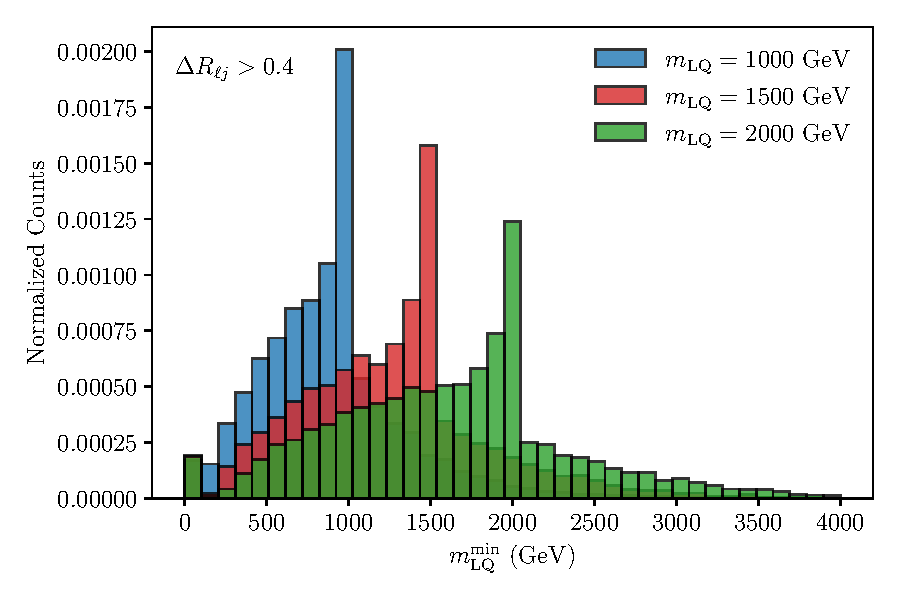
\includegraphics[width=0.85\textwidth]{figs/mLQ_mmin_histogram.pdf}
    \caption{Reconstructed minimum leptoquark mass $m^{\text{min}}_{\text{LQ}}$ distributions for three benchmark scalar leptoquark mass points: $m_{S_1} = 1.0, 1.5, 2.0~\text{TeV}$.
    The agent-orchestrated the full simulation chain (\textsc{FeynRules}, \textsc{MadGraph}, \textsc{Pythia}, jet clustering, and invariant mass reconstruction) for each scan point, producing resonance peaks centered at the corresponding generated masses.
    Each distribution contains 10,000 simulated events with symmetric two-body decay reconstruction $(\ell j)(\ell j)$ and $\Delta R > 0.4$ separation cuts.}\label{fig:resonance_reconstruction}
\end{figure}

The complete leptoquark mass-scan example illustrates how these components function together in practice. 
Beginning from a pre-initialized sandbox, the agent autonomously identified available model and run-card files, generated a UFO model with \textsc{FeynRules}, executed a parameter scan with \textsc{MadGraph}, and showered each mass point with \textsc{Pythia}. 
It then carried out jet clustering, object selection, and resonance reconstruction using schema-validated analysis tools. 
A notable feature of the workflow is the agent's ability to propagate scan metadata across stages without manual bookkeeping, recover from intermediate failures, and maintain a structured execution trace throughout without input from the user. 
The resulting minimum lepton-jet invariant mass distributions for the three signal benchmarks are shown in \cref{fig:resonance_reconstruction}, demonstrating that the orchestrated workflow successfully reconstructs the expected resonance peaks and produces reproducible, analysis-ready outputs.
\vspace{-0.1in}
\section{Conclusions}\label{sec:conclusions}

In this work, we introduced \pkgname, an orchestration framework that integrates large language models into HEP workflows. 
By treating scientific software as a collection of formally specified operations, \pkgname enables LLMs to coordinate domain-specific codes within transparent, human-supervised workflows. 
The complete leptoquark analysis demonstrated how these components combine to form a reproducible multi-stage pipeline spanning model definition, event generation, showering, reconstruction, and downstream analysis.

\pkgname{} complements the \orchestralai engine with HEP-specific abstractions, including schema-validated tools, run-card–driven configuration, and LLM-compatible event data structures. By treating run cards, intermediate artifacts, and structured event representations as first-class objects within a persistent orchestration loop, \pkgname{} provides a stable and auditable interface linking symbolic theory inputs, numerical configuration choices, and multi-stage simulation workflows. This design enables the seamless construction and execution of end-to-end HEP pipelines while preserving transparency, provenance, and human oversight throughout.

Looking forward, increasingly agentic scientific systems will likely play a growing role in HEP research. 
With reliable tool interfaces and structured context, LLM-driven agents could assist in tasks such as generator tuning, parameter-space exploration, automated background modeling, or adaptive analysis strategies that respond to intermediate results. 
More capable multi-agent configurations may support iterative model refinement, where one agent proposes theoretical extensions, another evaluates phenomenological viability, and a third orchestrates simulations to test consistency against data \cite{jiang2025agenticscimlcollaborativemultiagentsystems}. 
Such systems would not replace human judgment, but rather amplify it by automating the mechanical components of scientific computation while preserving interpretability and oversight.

The present architecture suggests several natural directions for future work.
First, run-card-based retrieval-augmented generation (RAG) offers a principled path toward more reliable configuration synthesis: curated collections of validated cards, parameter dictionaries, and tool-specific patterns could guide agents toward syntactically correct and semantically meaningful configurations without extensive supervision. 
A closely related extension is the automated extraction of phenomenological models from the literature. An agent could ingest a \texttt{hep-ph} manuscript, identify the relevant field content and interactions, and construct a corresponding \textsc{FeynRules} model file or an equivalent intermediate representation together with the other event-generator configurations, enabling end-to-end translation of theoretical models described in the literature to event-level simulations.
Second, extending the orchestration layer to closely related domains such as additional HEP event generators, \textsc{HepMC} \cite{Buckley:2019xhk} export, detector simulation, global analyses, and cross-generator validation represents the most direct progression from the capabilities demonstrated here. 
These additions would allow \pkgname{} to support full end-to-end phenomenological studies without altering the underlying orchestration philosophy.
Beyond these immediate extensions, \pkgname can also incorporate broader classes of HEP workflows, including neutrino event generators (e.g.~\textsc{Genie}\cite{Andreopoulos:2009rq}, \textsc{ACHILLES}\cite{Isaacson:2022cwh}), long-lived particle pipelines for beam-dump and intensity-frontier experiments, and detector-simulation interfaces for fixed-target and collider environments. 
Related opportunities include symbolic learning \cite{Alnuqaydan:2022ncd,Dong:2022trn}, model building \cite{Matchev:2024ash,Wojcik:2024lfy,Kawai:2024pws,Koay:2025bmu}, automating cross-generator consistency studies (e.g.~\textsc{Pythia}, \textsc{Sherpa}, \textsc{Herwig}), incorporating global-fit frameworks, or coordinating EFT-matching and parameter-inference tasks across multiple scales.
Third, progressively deeper forms of autonomy, such as agents that refine workflows in response to failures, track uncertainty across stages, or propose targeted simulations to resolve ambiguities, represent a promising evolution of the orchestration paradigm. In parallel, systematically logging agent decisions, tool invocations, and execution outcomes would enable the construction of domain-specific datasets for supervised fine-tuning and reinforcement learning, providing a path for improved agent performance through experience rather than prompt engineering alone. 

\pkgname provides the infrastructure required for these developments: a reliable, robust, auditable, and extensible orchestration layer through which future agentic systems can plan, execute, and refine HEP workflows. 
By linking symbolic theory to measurable data within a principled tool-driven environment, \pkgname offers a foundation for progressively more capable AI-assisted research in high-energy physics.

{\bf Acknowledgements.} The work of TM, AR and KM is supported in part by the Shelby Endowment for Distinguished Faculty at the University of Alabama. The work of SG is supported in part by the U.S. Department of Energy (DOE) under Awards No. DE-SC0012447 and No. DE-SC0026347. The work of KM is supported in part by the U.S. Department of Energy (DOE) under Award No. DE-SC0026347.
The work of TM is partially supported by Fermilab via Subcontract 725339. 
The work of AR and KM is partially supported by Fermilab via Subcontract 731293, in support of DOE Award No.\ DE-SCL0000090 ``HEP AmSC IDA Pilot: Knowledge Extraction'' and DOE Award No.\ DE-SCL0000152 ``USQCD AmSC Infrastructure Provision''.
PS is supported by the U.S. Department of Energy, Office of Science, Office of High Energy Physics QuantISED program under the grants ``HEP Machine Learning and Optimization Go Quantum'', Award Number 0000240323, and ``DOE QuantiSED Consortium QCCFP-QMLQCF'', Award Number DE-SC0019219.
This manuscript has been authored by Fermi Forward Discovery Group, LLC under Contract No. 89243024CSC000002 with the U.S. Department of Energy, Office of Science, Office of High Energy Physics.

{\bf Public code.} The open-source software developed for this project is publicly available at:
\begin{center}
{\url{https://github.com/tonymenzo/heptapod}}.
\end{center}

\newpage
\begin{appendix}

\section{Tools}
\label{app:tools}

This appendix summarizes the domain-specific tools made available to the agent.
Tools are grouped by their role in the workflow and provide a uniform, schema-validated interface.
All tools inherit from the \texttt{BaseTool} abstraction, which defines the interface between tools and the LLM orchestrator by converting type-annotated Python classes into LLM-compatible function schemas, separating runtime parameters (\texttt{RuntimeField}) from configuration state (\texttt{StateField}), and providing automatic validation and structured error handling (see \cref{sec:architecture} and \cite{orchestral-ai} for details).
Each tool entry below specifies its \emph{Purpose}, \emph{Inputs}, \emph{Behavior}, and relevant \emph{Notes}.
Full implementations and API documentation are available in the public repository.

\begin{table*}[p!]
\centering
\begin{sideways}
\begin{tabular}{llp{10cm}}
\hline
\textbf{Category} & \textbf{Tool} & \textbf{Purpose} \\
\hline
\multirow{3}{*}{Event Generation}
  & \texttt{FeynRulesToUFOTool} & Generate a validated UFO model directory from a \textsc{FeynRules} \texttt{.fr} file for use in matrix-element generators. \\
  & \texttt{MadGraphFromRunCardTool} & Execute \textsc{MadGraph5\_aMC@NLO} with runtime substitutions and automatic identification of parameter scans. \\
  & \texttt{PythiaFromRunCardTool} & Run \textsc{Pythia}~8 event generation or LHE showering/hadronization with JSONL event output. \\
\hline
\multirow{3}{*}{Data Conversion}
  & \texttt{LHEToJSONLTool} & Convert LHE events into the unified \texttt{evtjsonl-1.0} schema used throughout the workflow. \\
  & \texttt{EventJSONLToNumpyTool} & Convert particle-level JSONL into padded NumPy arrays suitable for ML and vectorized analysis. \\
  & \texttt{JetsJSONLToNumpyTool} & Convert jet-level JSONL collections into fixed-shape NumPy arrays with configurable feature sets. \\
\hline
Jet Clustering
  & \texttt{JetClusterSlowJetTool} & Cluster jets using anti-$k_T$/CA/$k_T$ algorithms via \textsc{Pythia}'s \texttt{SlowJet} interface. \\
\hline
\multirow{7}{*}{Kinematic Analysis}
  & \texttt{CalculateInvariantMassTool} & Compute invariant masses for user-specified combinations of particles. \\
  & \texttt{CalculateTransverseMomentumTool} & Extract transverse-momentum distributions from particle or jet collections. \\
  & \texttt{CalculateDeltaRTool} & Compute $\Delta R$ separations between objects in one or two collections. \\
  & \texttt{ApplyCutsTool} & Apply kinematic selections with user-defined thresholds. \\
  & \texttt{SortByPtTool} & Order objects by transverse momentum within each event. \\
  & \texttt{MergeObjectCollectionsTool} & Merge multiple JSONL object collections into a single event-aligned file. \\
  & \texttt{FilterByDeltaRTool} & Remove objects based on $\Delta R$ proximity to another collection. \\
\hline
\multirow{3}{*}{Event Selection}
  & \texttt{GetHardestNTool} & Select the $N$ highest-$p_T$ particles per event with optional species filtering. \\
  & \texttt{GetHardestNJetsTool} & Select the $N$ highest-$p_T$ jets per event from jet JSONL files. \\
  & \texttt{FilterByPDGIDTool} & Retain only particles with specified PDG IDs and report filtering efficiencies. \\
\hline
Advanced Analysis
  & \texttt{ResonanceReconstructionTool} & Perform physics-aware two-body mass reconstruction from multiple object collections. \\
\hline
\end{tabular}
\end{sideways}
\caption{Summary of the HEP orchestration tool suite exposed to the agent.}
\label{tab:tools}
\end{table*}

% ======================================================================
% Event Generation
% ======================================================================

\subsection{Event Generation}

\paragraph{\texttt{FeynRulesToUFOTool}.}
\textbf{Purpose.} Produce a complete and validated UFO model directory from a \textsc{FeynRules} \texttt{.fr} file, enabling subsequent use in \textsc{MadGraph}.
\textbf{Inputs.} Model file path, UFO output directory, optional \texttt{feynrules\_path}, \texttt{wolframscript} path, timeout.
\textbf{Behavior.} Executes an isolated \textsc{Mathematica} session to load the model and generate the UFO; verifies the resulting directory structure (particles, parameters, vertices, couplings).
\textbf{Notes.} Errors originating from model syntax or missing executables are surfaced with structured metadata to support agent-level recovery.

\paragraph{\texttt{MadGraphFromRunCardTool}.}
\textbf{Purpose.} Execute \textsc{MadGraph5\_aMC@NLO} using a template run card with runtime modifications, and present parameter scans in a uniform structured format.  
\textbf{Inputs.} Template \texttt{.mg5} file and optional overrides: UFO path, output name, event count, seed.  
\textbf{Behavior.} Rewrites the run card with substitutions, runs MG5, detects multi-run scans from MG5 output directories, and returns structured metadata per run (parameter values, LHE paths, cross sections, uncertainties).  
\textbf{Notes.} Single-run and multi-run cards are exposed to the agent through the same metadata schema.

\paragraph{\texttt{PythiaFromRunCardTool}.}
\textbf{Purpose.} Provide \textsc{Pythia}~8 event generation, including hard-process simulation, parton showering, and hadronization, with optional LHE input and standardized JSONL event output. Supports both fully standalone generation and LHE-based showering/hadronizing modes.
\textbf{Inputs.} Command card, number of events, seed, flags for final-state filtering, optional \texttt{shower\_lhe} flag and \texttt{lhe\_path}.
\textbf{Behavior.} Runs Pythia with the supplied configuration; outputs each event in the \texttt{evtjsonl-1.0} schema and records cross-section information from Pythia's statistics block. In LHE showering mode (\texttt{shower\_lhe=True}), applies parton showering and hadronization to pre-generated matrix-element events.
\textbf{Notes.} When showering LHE files, the tool automatically injects the appropriate \texttt{Beams:LHEF} directive with the absolute path to the LHE file.

% ======================================================================
% Data Conversion
% ======================================================================

\subsection{Data Conversion}

\paragraph{\texttt{LHEToJSONLTool}.}
\textbf{Purpose.} Convert LHE events into the unified JSONL event format used across the orchestration workflow.  
\textbf{Inputs.} LHE file path, output JSONL file path.  
\textbf{Behavior.} Parses all events and emits line-delimited JSON objects following the \texttt{evtjsonl-1.0} schema.  
\textbf{Notes.} Serves as a standardized bridge between matrix-element generators and downstream tools.

\paragraph{\texttt{EventJSONLToNumpyTool}.}
\textbf{Purpose.} Provide a fixed-shape NumPy representation of particle-level events for batch or ML processing.
\textbf{Inputs.} JSONL file, output directory.
\textbf{Behavior.} Identifies the maximum particle multiplicity and constructs an array of shape $(N_{\mathrm{events}}, N_{\mathrm{max}}, 5)$ with columns $[p_x,p_y,p_z,E,\texttt{id}]$ where $\texttt{id}$ is the PDG identifier.
\textbf{Notes.} Ensures deterministic shapes compatible with JAX, PyTorch, and NumPy.

\paragraph{\texttt{JetsJSONLToNumpyTool}.}
\textbf{Purpose.} Convert jet collections to fixed-shape NumPy arrays with configurable kinematic features.  
\textbf{Inputs.} Jet JSONL file, output directory, feature-extraction mode.  
\textbf{Behavior.} Extracts per-jet kinematics and optional auxiliary information; pads events to consistent shapes.  
\textbf{Notes.} Supports ML workflows requiring homogeneous jet representations.

% ======================================================================
% Jet Clustering
% ======================================================================

\subsection{Jet Clustering}

\paragraph{\texttt{JetClusterSlowJetTool}.}
\textbf{Purpose.} Perform jet clustering using anti-$k_T$, Cambridge/Aachen, or $k_T$ algorithms through \textsc{Pythia}'s \texttt{SlowJet}.
\textbf{Inputs.} Particle JSONL file, algorithm choice, radius $R$, $p_T$ threshold, $\eta$ range, \texttt{cluster\_all} flag, optional output path.
\textbf{Behavior.} Constructs Pythia event containers from JSONL inputs, applies the chosen algorithm, and outputs jet collections in JSONL format with full kinematics and constituent indices. When \texttt{cluster\_all=True}, processes entire dataset and streams results to the specified output file.
\textbf{Notes.} Supports both single-event and batch-processing modes for large datasets.

% ======================================================================
% Kinematic Analysis
% ======================================================================

\subsection{Kinematic Analysis}

\paragraph{\texttt{CalculateInvariantMassTool}.}
\textbf{Purpose.} Compute invariant masses for user-specified particle combinations within each event.  
\textbf{Inputs.} Particle JSONL file, index selections.  
\textbf{Behavior.} Computes $m=\sqrt{E^2 - \vec p^{\,2}}$ for each combination and writes results to JSON.  
\textbf{Notes.} Integrates with selection tools for higher-level analyses.

\paragraph{\texttt{CalculateTransverseMomentumTool}.}
\textbf{Purpose.} Extract particle or jet transverse-momentum distributions.  
\textbf{Inputs.} JSONL file.  
\textbf{Behavior.} Computes $p_T=\sqrt{p_x^2+p_y^2}$ for all objects and outputs per-event lists.  

\paragraph{\texttt{CalculateDeltaRTool}.}
\textbf{Purpose.} Compute angular separation between objects in one or two collections.  
\textbf{Inputs.} One or two JSONL collections; optional matching strategies.  
\textbf{Behavior.} Returns $\Delta R$ for all relevant pairs.  

\paragraph{\texttt{ApplyCutsTool}.}
\textbf{Purpose.} Apply user-defined kinematic cuts to particle or jet collections.  
\textbf{Inputs.} JSONL file, cut definitions.  
\textbf{Behavior.} Evaluates cuts per event and outputs the filtered JSONL file.  

\paragraph{\texttt{SortByPtTool}.}
\textbf{Purpose.} Sort objects by transverse momentum within each event.  
\textbf{Inputs.} JSONL file.  
\textbf{Behavior.} Computes $p_T$ and sorts objects in descending order.  

\paragraph{\texttt{MergeObjectCollectionsTool}.}
\textbf{Purpose.} Combine multiple object collections into a single event-aligned JSONL file.  
\textbf{Inputs.} List of JSONL files.  
\textbf{Behavior.} Merges per-event objects while preserving event IDs.  

\paragraph{\texttt{FilterByDeltaRTool}.}
\textbf{Purpose.} Remove objects based on $\Delta R$ proximity to objects in other collections, enabling overlap removal and isolation criteria.
\textbf{Inputs.} List of JSONL files containing pre-selected objects, $\Delta R$ threshold, filter mode (\texttt{remove\_first}, \texttt{remove\_second}, \texttt{remove\_both}, \texttt{keep\_only\_separated}), optional output paths.
\textbf{Behavior.} Applies $\Delta R$ constraints only between objects from different input arrays; objects within the same array are never constrained by this criterion. Permanently removes objects that fail the separation requirements and outputs filtered collections.
\textbf{Notes.} Common use cases include jet-lepton overlap removal and lepton isolation. Distinct from \texttt{ResonanceReconstructionTool}: this tool permanently removes objects and is not suitable for analyses requiring object pairing such as resonance mass reconstruction.  

% ======================================================================
% Event Selection
% ======================================================================

\subsection{Event Selection}

\paragraph{\texttt{GetHardestNTool}.}
\textbf{Purpose.} Select the $N$ highest-$p_T$ particles per event, optionally restricted by PDG ID.  
\textbf{Inputs.} Particle JSONL file, $N$, optional PDG list.  
\textbf{Behavior.} Computes $p_T$, ranks objects, and retains the top $N$.  

\paragraph{\texttt{GetHardestNJetsTool}.}
\textbf{Purpose.} Select the $N$ highest-$p_T$ jets per event from jet JSONL files.
\textbf{Inputs.} Jet JSONL file (with \texttt{data.jets} schema from \texttt{JetClusterSlowJetTool}), $N$.
\textbf{Behavior.} Orders jets by $p_T$ and retains the leading $N$.
\textbf{Notes.} Designed specifically for jet collections; for particle-level objects, use \texttt{GetHardestNTool} instead.  

\paragraph{\texttt{FilterByPDGIDTool}.}
\textbf{Purpose.} Filter particle collections to retain only specified PDG IDs.  
\textbf{Inputs.} JSONL file, PDG list.  
\textbf{Behavior.} Applies per-event filtering and reports efficiencies.  

% ======================================================================
% Advanced Analysis
% ======================================================================

\subsection{Advanced Analysis}

\paragraph{\texttt{ResonanceReconstructionTool}.}
\textbf{Purpose.} Perform $n$-body resonance reconstruction from multiple object collections using physics-aware pairing templates.
\textbf{Inputs.} Lists of JSONL files (e.g., leptons and jets), optional minimum $\Delta R$ separation (\texttt{min\_delta\_r}), mass-pairing template (\texttt{two\_body\_symmetric} or \texttt{n\_body\_all\_pairs}).
\textbf{Behavior.} Evaluates all allowed disjoint pairings consistent with the template, selects the pairing minimizing $|m_1 - m_2|$ (for symmetric template), and outputs per-event mass observables in \texttt{.npy} format with summary statistics and histograms.
\textbf{Notes.} When \texttt{min\_delta\_r} is specified, $\Delta R$ constraints apply \emph{only across input collections} (e.g., lepton-jet separation), not within collections (e.g., lepton-lepton or jet-jet pairs are unconstrained). Pairings that combine only same-collection objects are automatically rejected when multiple collections are provided with active $\Delta R$ constraints, ensuring physically meaningful resonance reconstruction.

\end{appendix}

\newpage
\bibliography{ref}{}
\bibliographystyle{JHEP}

\end{document}
